\documentclass[12pt,a4paper]{report}
\usepackage[utf8]{inputenc}
\usepackage{graphicx}
\usepackage{wrapfig}
\usepackage{tikz} 
\usepackage{float} 
\usepackage{pgf-umlcd} 
\usepackage{pgf-umlsd} 
\usepackage{listings}

\renewcommand{\chaptername}{}

\title{
Final Report - ESCiMO \\
in \LaTeX{}
}

\author{
Joris Vergeer - 1585591\\
Gerben Boot - 1575754\\
\\
\\
Daniel Telgren
}

\begin{document}
\maketitle

\begin{abstract}
%%
%%TODO Rewrite parts of this
%%
Grid Manufacturing (GM) is a new production paradigm, based upon the use of standardized and modular Reconfigurable Manufacturing Systems (RMS).\cite{SICE13}
A production unit in a RMS is called an equiplet.
Each equiplet contains interchangeable modules. 
These hardware modules have software counterparts.
In this report we look at the realisation of the state machines build into the software counterparts of modules and equiplets as well as the realisation of a SCADA for the equiplet with its modules.
\end{abstract}

\tableofcontents


\chapter{Introduction}
In the 6th semester of our course Computer Science at the University of Applied Science Utrecht we participated in the Ubiquitous Computing specialisation.

\subsubsection{Agile/Grid manufacturing}
To meet the requirements of modern production, where short
time to market, requirement-driven production and low cost
small quantity production are important issues, we have de-
veloped a production hardware infrastructure as well as an
agent-based software infrastructure for agile industrial pro-
duction. This production is done on special devices called
equiplets. A grid of these equiplets connected by a fast net-
work is capable of producing a variety of different products
in parallel. The multi-agent-based software infrastructure is
responsible for the agile manufacturing.\cite{Paper70}

\subsubsection{Equiplet}
The Equiplet is a part of the Agile/Grid manufacturing. The Agent consist of multiple agents and controls one or more modules. Based on the connected modules of the equiplet, provide the equiplet services for an other agent in the Agile/Grid manufactoring environment. 
\paragraph{Agent}
The equiplet agent is the leading agent for the equiplet. It is responsible for negotiation with the product agent and managing the equiplet schedule.\cite{REXOS_Design}
\paragraph{Service Agent}
The service agent is responsible for translating a product step into service step(s). The service agent also represents equiplet services based on the attached modules. The set of product steps which can be performed is based on the services it provides.\cite{REXOS_Design}
\paragraph{Hardware Agent}
The hardware agent is responsible for the interaction with the ROS layer. It translates service steps into equiplet steps, which can be interpreted by the ROS layer. It has a specific piece of software for each hardware module that is currently attached to the equiplet. Each one of these pieces of software is responsible for its own hardware module on the equiplet, and handle the actual translation. Each service step has a specific module that will lead the translation. \cite{REXOS_Design}
\paragraph{ROS Equiplet}
The ros equiplet is the responsible for the control of a set of modules which belong to by the equiplet. This equiplet part works with the the ROS system.

\subsubsection{Module}
An module is an part of the system which controls one or more devices. This part can be seen as the lowest layer of the hardware control. A distinction is made between modules that contain parts that are potentially dangerous and modules that do not contain these parts. These parts are, amongst others, all moving parts,parts that heat up, parts that eject matter and parts that emit electromagnetic radiation. Modules that contain any of these parts are known as actors. Their counterparts (modules that are not potentially dangerous) are nonactors.\cite{mast_funcional_design}

\subsubsection{Blackboards}
The Agile Manufacturing contain of three blackboard:Product steps,Service steps and Equiplet steps. These blackboard will be used to communicate between the equiplet agents or to communicate with the ROS node. All these blackboard steps contain a state, about the progress of the step:EVALUATING, PLANNED, WAITING, IN PROGRESS, SUSPENDED/WARNING, DONE, ABORTED and FAILED.

\subsubsection{State Machine}
A finite-state machine (FSM) or finite-state automaton (plural: automata), or simply a state machine, is a mathematical model of computation used to design both computer programs and sequential logic circuits. It is conceived as an abstract machine that can be in one of a finite number of states. The machine is in only one state at a time; the state it is in at any given time is called the current state. It can change from one state to another when initiated by a triggering event or condition; this is called a transition. A particular FSM is defined by a list of its states, and the triggering condition for each transition.\cite{state_machine}

\subsubsection{Equiplet, SCada, MOdules (ESCiMO)}
In our ubiquitous computing project we are developing a system to control a production unit in an RMS called equiplet. 

Equiplets contain interchangeable modules. 
You can reconfigure an equiplet by changing its modules.
Because modules can be changed on the fly, the equiplet has to dynamically adapt to its new configuration.
Due to the autonomous nature of equiplets they can receive instruction at any time.

This together creates a lot of problems we have to solve.


\chapter{Project team}
The following people have worked on ESCiMO

\begin{tabular}{l | l}
Name       & Role \\
\hline
D. Telgren & Project supervisor \\
G. Boot    & Software developer EST, MOST \\
J. Vergeer & Software developer SCADA, MOST
\end{tabular}


\chapter{Assignment}
\section{Problem description}
\subsection{Safety}
Equiplets are autonomous machines. 
They are part of a large production platform where multiple entities can request actions form the equiplet.
These requests can be received at any time.
Even when an operator is working on an equiplet.
When an operator is working on an equiplet, it has to be absolutely safe.
Modules must be powered off and have to be guarantee that they will not power up while the operator is still nearby.
To prevent this a safety mechanism has to be build.
\subsection{Synchronisation}
When instructions require actions from multiple modules both modules have to be ready.
Modules are not guaranteed to be ready at the same time. Some modules require initialisation  and/or calibration procedures while other modules are immediately ready.
To prevent instructions to be send to modules which are not ready yet a synchronisation mechanism has to be build
\subsection{Error handling}
Modules can break down during operation. When this happens the equiplet must abort its current instruction and stop receiving new instructions until the module is fixed.
\subsection{Human interaction}
Some times a human want to have control to the equiplet. There are different options for humans to influenced the system such as an emergency button or by an step button to execute tasks by press on a button.

\subsection{SCADA}
To operate an equiplet the operator has to be able to see what is going on with the equiplet and modules. He also want an interface where he can perform minimal interaction with the equiplet. Therefore also a SCADA system has to be developed.

\section{Goals}
\begin{itemize}
\item Research current State Machine
\item Improve current State Machine with missing elements
\item Implements designed State Machine in Agile/Grid manufacturing project 
\item Design and implement SCADA of the equiplet
\end{itemize}

\newpage
\section{Requirements and conditions}

\subsection{State Machine}
\subsubsection{Modes as additional of the State Machine}
Mode is an additional of the State Machine to implement the missing elements.
Currently the State Machine contains of states and transitions. A mode is a new dimension at the State Machine. In this case the State Machine react depended on its state and also on its mode.
\paragraph{Emergency Stop}In this mode the modules has lost the devices control and it is possible to show the State Machine as safe.
\paragraph{Error}The error is intended for non-actor modules which in error. The State Machine may not allowed to startup. When a module in error and the State Machine in Normal, the module must try to finish it task and go to standby by stop.
\paragraph{Critical Error}The Critical error mode is intended for actor modules which in error. When an actor module in error, the module should stop when in normal and shutdown when in standby.
\paragraph{Service}The Service mode will be used to add configuration calls to the module. In this mode the repairer should be used this calls.

\subsection{Equiplet additions}
\subsubsection{Module control}
\paragraph{Emergency Stop}
When the emergency button is pressed, the equiplet can't execute equiplet steps, because the hardware of the modules are offline.
\paragraph{Module in Error}
When a module in error (this means a non-actor module) the other modules must try to finish its task if running. It is possible to run new tasks without the module which in error, but this is not usual said by Erik Puik. He prefer that an equiplet only runs tasks which use all its modules, so the equiplet will always full use its components(modules) and is attractive to the market. In this case we can say when an module in error, the equiplet is also in error.
\paragraph{Module in Critical Error}
When a module in critical error (this means a actor module) the other modules must abort its task and stop/shutdown. In this case an actor module constitutes a risk so the modules of the equiplet must shutdown to safe.

\subsubsection{Equiplet opportunities}
\paragraph{Step control}
The equiplet should execute exeplet steps by once named as 'Step control'.

\subsubsection{Equiplet reaction on module State Machine changes}
When the modules of the equiplet are not ready, it isn't possible to execute equiplet steps. In this case the equiplet must change the states of the equiplet steps. It is out of the scope to change this states, but the equiplet must know all module states to react on it.

\newpage
\section{Final products}
\subsection{State Machine}
Our first product is a state machine for modules and equiplets. 

In addition to states, there are also modes.
A mode defines which states and transitions are allowed.

\subsubsection{MOdule STatemachine (MOST)}
The module state machine is an expansion of MAST with modes.
The state machine is our solution for the error handling, safety guarantee and synchronisation.

\subsubsection{Equiplet STatemachine (EST)}
The EST variant of the state machine is implemented in the equiplet.
It has additional functionality for managing registered MOST state machines and also include modes.

\subsection{SCADA}
The SCADA gives operators insight into the equiplet.
It shows the current state and modes of the equiplet and its modules.
It also gives the operator some control over the equiplet.
In the SCADA he can change the mode and state of the equiplet and its modules.

\subsection{Implementation}
Finally we will implement the state machines in existing modules and equiplets.

\subsection{Documentation}
\paragraph{Project Transfer Document}We also make a Project Transfer Document with the parts of our design and describe what is done and what remains to be done.

\chapter{Analysis}
\section{StateMachine}
\begin{wrapfigure}{r}{0.35\textwidth}
	\begin{center}
		\includegraphics[scale=0.5]{pictures/mast.png}
	\caption{MAST}
	\vspace{-100pt}
	\end{center}
\end{wrapfigure}
For the Agile/Manufacturing is a State Machine designed. This State Machine consist of states and transitions. Transitions which set the State Machine to an higher state, has also an abort state to return. The State Machine is intended to control the hardware.
\subsection{States}
The state machine will have three states:
\begin{itemize}
\item \textbf{Safe} I.e. safe for an human.
\item \textbf{Standby} I.e. the machine will be ready to run, but isn’t running.
\item \textbf{Normal} I.e. the machine is in progress.
\end{itemize}
\newpage
\subsection{Transition states}
Between the states there are transition states, which is the only way to change from state. Transition states are responsible to set the machine correct to the next state according the state requirements.  
There are four transition states:
\begin{itemize}
\item \textbf{Setup} to change from safe to standby
\item \textbf{Shutdown} to change from standby to safe
\item \textbf{Start} to change from standby to normal
\item \textbf{Stop} to change from normal to standby
\end{itemize}

\subsection{Abort Transition}
It will be possible that in a transition state the transition will be undo. This is possible by an abort transition. When the machine in a transition state and the transition must be aborted, the transition must stop its commands and change from state to its contrary state. 
The next aborts transitions are possible:
\begin{itemize}
\item Setup to Shutdown
\item Start to Stop
\end{itemize}

\subsection{Implementation}
The StateMachine class has a transitionMap that is used to find the transition function that belongs to the transitions state. This way, a transition function can only be called when it’s in the map. So a direct transition from safe to standby without going through setup is impossible. The state machine class contains all the logic for receiving state change request and sending the state update messages to the EquipletNode. The module classes only need to implement the the transition functions. Those are module specific so the state machine can’t define those. So it’s the programmer’s responsibility to implement the transitions properly.
\\\\
This is a basic implementation of the state machine in REXOS. In the current version of the software, when an error occurs the node will crash rather than transition to a lower state so that the system can recover.\cite{mast_technical_design}

\newpage
\section{MOdule STateMachine (MOST)}
The State Machine is implemented by modules. This implemented StateMachine is called MOST.

\subsection{Transition states}
The transition states set the module to the next state. Each Transition must be implemented in the module, because different modules has different transition implementation.

\paragraph{Setup}This transition could be used for: calibration, preheat etc.
\paragraph{Shutdown}This transition could be used for: less power of motors, cool down etc.
\paragraph{Start}The module receive equiplet step data to execute
\paragraph{Stop}This transition could be used to set the module on its Standby position.

\subsection{Implementation}
The modules implement the state machine by extending the StateMachine superclass. The state machine class has virtual transition functions that need to be implemented in the module when it extends the superclass.
\\\\
The state of the module can be changed by an changeState method which is implemented in the State Machine.

\newpage
\section{The equiplet states}
Due to the nature of the (autonomous) modules in the reconfigurable system the modules can have states that differ from one another. The equiplet node is the central point in which all modules are known. The equiplet itself has two states, one to monitor safety and one to monitor operation. Each state depends on the states of the modules attached to the equiplet in its own
way.
\textbf{The safety state} indicates the level of safety and is equal to the highest actor module state.
\textbf{The operation state} indicates whether the equiplet is able to fulfill the current task and is equal to the lowest state of the required modules. The required modules are the modules necessary tofulfill the current task as known by the hardware agent.\cite{mast_funcional_design}

\newpage
\section{Missing elements}
\subsection{MAST}
The current State Machine MAST which the Modules implemented miss some required functionality. These missing have been described here.
\subsubsection{Emergency button}
A module has always an emergency button to guarantees safety. When the emergency button is pressed, the software must react on it.
\subsubsection{Errors}
Modules can break down during operation. When this happens it should not receive more tasks from the equiplet to execute. Also its current tasks can not finish.
\subsubsection{(Re-)configuration}
The current state-machine hasn't options to switch to an position to (re-)configurate or to switch to a mode of repair. An repair would see more technical information about the hardware executions and want to reconfigure.
\subsubsection{Lock}
A human would the option to lock on a state of the state machine such as to lock on safe or standby. Lock will means that it isn't possible to call transitions. When the human lock on safe, it guarantees that the state machine hold the safe position.
\subsection{Equiplet control}
\subsubsection{Equiplet node}
\paragraph{Modules}The equiplet controls one or more modules. All modules implement a State Machine, but the equiplet must react on changes of the State Machine of the modules.
\paragraph{Equiplet Step}When a module in error, the equiplet should to stop executing its current equiplet step and set it on an aborted state. This option is possible, because all blackboard steps contains states. 
\\Also when a module in error there are two options:
\begin{enumerate}
\item Stop executing equiplet steps
\item Stop executing equiplet steps which needed the module which in error.
\end{enumerate}
In both cases, the equiplet must react when a module in error
\subsubsection{Equiplet Agent}
The equiplet agent must know when the equiplet node has all modules in standby. Also when modules has an error, the equiplet should react on it such as to schedule no more.
\subsubsection{Equiplet Step Control}
Some equiplet has a (mostly)yellow button. This button should be needed to execute equiplet steps by once and execute next by a press on the button.

\chapter{Design}
\section{State Machine included mode}
\begin{wrapfigure}{r}{0.5\textwidth}
  \vspace{-30pt}
  \begin{center}
    \includegraphics[width=0.48\textwidth]{pictures/StateMachine_mode.png}
  \end{center}
  \vspace{-20pt}
  \caption{StateMachine overview}
  \vspace{-10pt}
\end{wrapfigure}
The State Machine is now renewed whit the new mode part. First the State Machine was controlled by its state. Now the State Machine can be controlled by its state and its mode.

\subsection{Mode change}
Currently there is no transition between a mode change. Also it is possible to all modes independent of its current mode. Perhaps this should implemented in the future to control the mode changes, but now it isn't necessary.

\subsection{State Machine addition}
The State Machine add functionality to influence the State Machine. This should be needed by modes. Each mode is designed by possible states and possible transitions.
\paragraph{Possible (transition)states}When the State Machine is in an non possible state, it abort. The abort of a transition state is it's contrary. The stop and shutdown transitions hasn't abort transitions. The abort of a state is it's lower transition state, such as: Normal=Stop and Standby=Shutdown. The Safe sate hasn't a abort.
\paragraph{Possible transitions}The State Machine change to an transition state only when it is in the possible transitions. If it isn't it is also not possible to change the state by this transition.

\subsection{Modes}
\includegraphics[width=1\textwidth]{pictures/modes.png}\\
The equiplet used different standard modes which influence the State Machine. Each mode discribe the possible states and transitions. All states and transitions which are not in the possibles are non possible. 

\subsubsection{Normal}This mode will mean that the State Machine runs in original mode. There are no particularities in this mode.\\\\
\textbf{Possible (transitions)states:}Normal, Standby, Safe, Setup, Shutdown, Start, Stop\\
\textbf{Possible transitions:}Setup, Shutdown, Start, Stop

\subsubsection{Service}This mode will be used to have more control of the machine. It can be used to (re-)configurate the machine or to get debug information. In this mode the State Machine is allowed to executed as in the normal mode.\\\\
\textbf{Possible (transitions)states:}Normal, Standby, Safe, Setup, Shutdown, Start, Stop\\
\textbf{Possible transitions:}Setup, Shutdown, Start, Stop

\subsubsection{Step}This mode will means that Step control is enabled. The State Machine runs it's task by once and continue when a user set the next step.\\\\
\textbf{Possible (transitions)states:}Normal, Standby, Safe, Setup, Shutdown, Start, Stop\\
\textbf{Possible transitions:}Setup, Shutdown, Start, Stop

\subsubsection{Error}This mode is used when an error is on the machine, but it isn't a dangerous error for the machine. When the module in Normal it should to stop and it task and it isn't allowed to start a new task when in Standby.\\\\
\textbf{Possible (transitions)states:}Standby, Safe, Setup, Shutdown, Stop\\
\textbf{Possible transitions:}Setup, Shutdown, Stop

\subsubsection{Critical Error}This mode is used when a dangerous error is detected on the machine. Only the Safe state is possible in this state and when the State Machine isn't safe, it should force to Stop if necessary and Shutdown.\\\\
\textbf{Possible (transitions)states:}Safe, Shutdown, Stop\\
\textbf{Possible transitions:}Shutdown, Stop

\subsubsection{Emergency Stop}This mode should used when the emergency stop is pressed. In this mode the State Machine is set as safe, because an emergency stop isn't a software stop but a hardware stop.\\\\
\textbf{Possible (transitions)states:}Safe\\
\textbf{Possible transitions:}-

\subsubsection{Lock}This mode is used to lock a state in the State Machine. This is simply realized to remote the transitions, but only the the Stop transition has remained. When it has finish its task it isn't possible to stay in normal, because the normal state will means that the machine is running. On this reason the stop transition is possible in this mode. When the machine is in a transition state it should finish it transition\\\\
\textbf{Possible (transitions)states:}Normal, Standby, Safe, Setup, Shutdown, Start, Stop\\
\textbf{Possible transitions:} Shutdown, Stop

\section{Module}
The module create a Module StateMachine called as MOST(MOdule STate machine). This State Machine extends from the designed State Machine, but implement the State Machine with predefined modes. When a module extends the Module State Machine it must indicate if it is an actor or not. This is used to set the module in error, which will be done by the Module State Machine. An actor module set the State Machine in the 'critical error mode' and a non actor module set it in the 'error mode'. 

\subsection{MOST modes}
\paragraph{Normal}The normal State Machine mode.
\paragraph{Service}When the module in Service, it enable debug information and it allowed service methods to calibrate etc.
\paragraph{Error}This mode is used when an non actor module in error.
\paragraph{Critical error}This mode is used when an actor module sets an error. The State Machine will go to the safe.
\paragraph{Emergency error}This mode is used when the emergency button is pressed

\section{Equiplet}
\subsection{State Machine}
The equiplet use also a State Machine to control the modules. This State Machine is calles EST(Equiplet STate machine). The EST should be implemented in the ROS node.

\subsubsection{States}
\paragraph{Safe}The equiplet is safe when all modules are also safe.
\paragraph{Standby}The standby state can be used when the modules of the equiplet in standby state. Just as the module standby state indicate this a ready for run. This state is imported for the equiplet because when the equiplet isn’t ready to run, it isn’t possible to perform scheduled tasks directly. This is designed by the requirement of Erik Puik that an equiplet only is ready to run when all modules are ready to run. When an module isn't ready to run, the equiplet should now allowed to run.
\paragraph{Normal}This state is used when the equiplet is executing an service step, i.e. the modules of the equiplet are running the equiplet steps. 

\subsubsection{Transitions}
\paragraph{Setup}Send to all modules of the equiplet a change state to standby command. This transition is finished when all modules are standby.
\paragraph{Shutdown}Send to all modules of the equiplet a change state to safe. This transition is finished when all modules are safe.
\paragraph{Start}It is starting a new service step and send the first equiplet step to the module. When the module is normal, this transition finished.
\paragraph{Stop}It is stopping the service step. When all modules are standby the equiplet change also to standby.

\subsubsection{Modes}
\paragraph{Normal}This mode is running when also all modules are normal
\paragraph{Service}When this mode is activated it set all modules in service.
\paragraph{Lock}This mode is to lock the equiplet.
\paragraph{Step}This mode execute an equiplet step by once. It send a new equiplet step to a module when the EquipetStateMachine receive an next step command.
\paragraph{Emergency error}This mode is used when the emergency button is pressed
\paragraph{Error}The equiplet activate this mode when a module is in error
\paragraph{Critical Error}The equiplet activate this mode when a module is in critical error.

\subsection{State Blackboard}
To provide equiplet agents from inform of the EST a blackboard should be used called the 'StateBlackboard'. This blackboard should be also used to allow the agent to change the state. The StateBlackboard provide the fallowing collections:
\paragraph{EquipletState}This collections contain the equiplet states. It provides the 'safety state', the operational state and the equiplet state. The safety- and the operational state provide only a state. The equiplet state provide a equiplet id, state and mode. 
\paragraph{EquipletCommands}By this blackboard the equiplet state can be changed.
\paragraph{ModuleStates}This collection contains all module states. A module state contain of a: module id, module state and the module mode.

\subsection{Overview}
Now the Equiplet contains the fallowing states:
\begin{itemize}
\item Safety state which is the highest state of all modules
\item Operational state which is the lowest state required modules of a service step.
\item It's own Equiplet State provides from the Equiplet State Machine
\end{itemize}

\section{SCADA}
\includegraphics[width=1\textwidth]{pictures/SCADA.png}
The E-SCADA runs on the equiplet PC and is a visual representation of everything happening in the equiplet. 

\subsubsection{Equiplet information}
\begin{itemize}
\item Name/ID
\item Safety state
\item Operational state
\item Equiplet state
\end{itemize}
\subsubsection{Equiplet control}
\begin{itemize}
\item Make the equiplet safe
\item Lock module
\item Continue step (step modi)
\end{itemize}
\subsubsection{Module information}
\begin{itemize}
\item Name/ID
\item Type
\item State
\item Modi
\end{itemize}
\subsubsection{Module control}
\begin{itemize}
\item Change module modi
\item Service information
\item Available services
\end{itemize}
\subsubsection{Scheduled services}
\begin{itemize}
\item Needed modules
\item Equiplet steps
\item Progress
\item Service state
\end{itemize}

\chapter{Final product}
\section{Result}
\subsection{MOST}

\begin{wrapfigure}{r}{0.5\textwidth}
    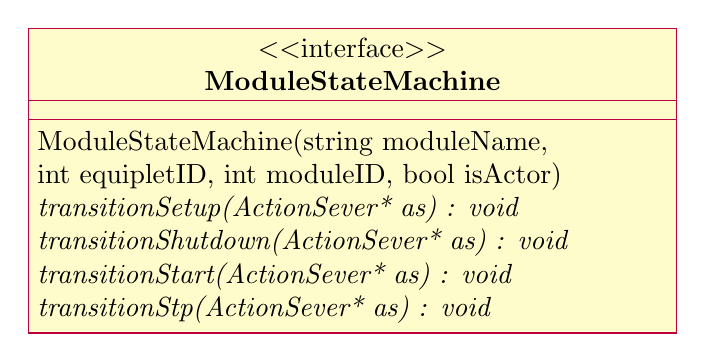
\begin{tikzpicture}
        \begin{interface}[text width=8cm]{ModuleStateMachine}{0,0}
        \operation{ModuleStateMachine(string moduleName, int equipletID, int moduleID, bool isActor)}
        \operation[0]{transitionSetup(ActionSever* as) :     void}
        \operation[0]{transitionShutdown(ActionSever* as) : void}
        \operation[0]{transitionStart(ActionSever* as) : void}
        \operation[0]{transitionStp(ActionSever* as) : void}
        \end{interface}
    \end{tikzpicture}
\end{wrapfigure}

MOST is a state machine for modules.
It is available as interface.
Each module has to implement it. 

The constructor of the ModuleStateMachine asks four parameters. \\
\\
\textbf{\textit{moduleName}} is the name of the module \\
\textbf{\textit{equipletID}} is the id of the eqiplet the module is attached to \\
\textbf{\textit{moduleID}} is the id of the module itself \\
\textbf{\textit{isActor}} is a boolean indicating of the module is an actor or not. \\

\noindent
The MOST implementation consists of four methods.
Each method represents a transition.
At the end of a transition the module has to call setSucceeded or setFailed on the given ActionServer.

\begin{figure}[H]
\begin{lstlisting}[language=c++, frame=single, caption=Sample transition]
void ModuleImplementation::transitionSetup(
	rexos_statemachine::TransitionActionServer* as) 
{
	ROS_INFO("Setup transition called");

	//Do groundbreaking initialisation sequence

	as->setSucceeded();
}
\end{lstlisting}
\end{figure}

\noindent
The state machine also takes care of registering itself at the equiplet. 
When a module starts it waits for an equiplet with the ID given in the state machines constructor. 
Then it will send a module registration request. 
The equiplet will then respond with a success or failure. 
If the registration has failed, the module will shut itself down.

\begin{center}
\begin{sequencediagram}
    \newinst{module}{:Module}
    \newinst{equiplet}{:Equiplet}
    \begin{call}{module}{ModuleRegistration(moduleName, moduleID)}{equiplet}{succeed}
    \end{call}
\end{sequencediagram}
\end{center}

\noindent
After registration EST has control over the states and modes of the module.

\subsection{EST}
EST is the state machine in the equiplet. 
This state machine has predefined functionality and is implemented for the greatest important parts.

EST controls the state and mode of the equiplet.
It also manages the state and modes of its attached modules.
EST provides the module registration functionality.

\subsection{State machine}
Both EST and MOST are based on the same base state machine. 

The base state machine provides a shared interface for controlling the state machine.
The interface consists of two ROS Actionlib actions for changing the desired state and mode.

\subsubsection{Modes}
The base state machine also defines some modes. Each essentially allows or disallows certain states and transitions.

When a change mode action is received and the current state is not allowed in the new mode, the state machine will force the module or equiplet to go to a allowed state.

\begin{figure}[H]
\caption{
    Example forced state change.
    Module is in normal state.
}
\begin{center}
\begin{sequencediagram}
    \newinst[0]{e}{:Equiplet}
    \newinst[5]{s}{:Statemachine}
    \newinst[1]{m}{:Module}
    \begin{messcall}{e}{changeMode(CRITICAL\_ERROR)}{s}
    \end{messcall}
    \begin{messcall}{s}{modeChanged(CRITICAL\_ERROR)}{e}
    \end{messcall}
    \begin{call}{s}{transitionStop}{m}{SUCCESS}
    \end{call}
    \begin{messcall}{s}{stateChanged(STANDBY)}{e}
    \end{messcall}
\end{sequencediagram}
\end{center}
\end{figure}

\subsection{SCADA}
SCADA runs in the same program that is running EST. 
EST provides SCADA with the information it needs. 
SCADA in turn uses EST to send commands to the registered modules.

\begin{figure}[H]
\begin{center}
\includegraphics[scale=0.4]{scada.png}
\end{center}
\end{figure}

\newpage
\section{Recommendations}

\chapter{Process and planning}
\section{planning}

\newpage
\section{Project Evaluation}
\subsection{Planning}
In the beginning an initial planning was made. 
After a couple of months the initial planning did not corresponds to new developments and has to be renewed.
Soon the planning became obsolete again and work started to be done on a priority base.

\subsection{Expectations}
In the end the project turned out to be more difficult than initially expected.
In the beginning the expectation were that only a state machine must be developed.
After some discussions and meetings with the project owners the whole project was unexpectedly up-scaled and redefined.

\subsection{Bottlenecks}
\subsubsection{Information gathering}
One of the biggest bottlenecks was information gathering.
It took a lot of time before it was clear what was expected.

\subsubsection{Improper use of project space}
For the project there was a room reserved where people who work on the project could work quietly.
However some teachers felt that that room was in ideal place to asses projects involving buzzers from students from earlier years.
This made the workplace busy and noisy.
Some days it was so noisy that other workplaces had to be found.

\subsection{Setbacks}
After a month of gathering information and creating a design that would satisfy all reasonable use cases it became clear that Erik Puik just wanted to see his idea back.

\subsection{Teamwork}
The teamwork was good. 
Each of the team-mates was skilled in other areas.
This resulted in some discussions form now and then.

\chapter{Reflection}
\section{Reflection technical competences}

\newpage
\section{Reflection professional competences}

\newpage
\section{Profile sketch}

\chapter{Abbreviations and concepts}
bron:[Project Transfer Document] Overview]
\subsubsection{ROS}
The Robot Operating System is an open source meta-operating system, designed to run on top of linux (Ubuntu): “It provides the services you would expect from an operating system, including hardware abstraction, low-level device control, implementation of commonly-used functionality, message-passing between processes, and package management. It also provides tools and libraries for obtaining, building, writing, and running code across multiple computers.”[32]
\subsubsection{Agent}
“The word ‘agent’ comes from the Latin word ‘agere’, meaning: ‘to act’. Software agents are autonomous entities[28] that have their own purpose and the ability to communicate with other agents. There are many definitions of a software agent, we prefer the definition of Wooldridge and Jennings[29] “An agent is an encapsulated computer system that is situated in some environment and that is capable of flexible, autonomous action in that environment in
order to meet its design objectives”.”[27]
\subsubsection{Mas}
“A multi-agent system (MAS) is a system composed of multiple interacting intelligent agents within an environment. Multi-agent systems can be used to solve problems that are difficult or impossible for an individual agent or a monolithic system to solve. Intelligence may include some methodic, functional, procedural or algorithmic search, find and processing approach.”[30]
\subsubsection{Grid}
A grid is a controlled group of equiplets.
\subsubsection{Equiplet}
An Equiplet is a product, the hardware, the "generic" modular machine (the HUniplacer is a prototype "instance" of an Equiplet type machine). An equiplet consist of one or more hardware parts which he is able to perform tasks.
\subsubsection{Module}
An module control some hardware parts of the equiplet. It is an subset of hardware devices of the equiplet.
\subsubsection{Device}
An device is an hardware element which produce information(sensors) or is able to execute tasks(actors).
\subsubsection{Blackboard}
bron:[Technical Design] Blackboard system
A blackboard is a structure for saving data and can be implemented as a database. It can also be used as a communication medium (e.g. a component submits a message to the blackboard and another component reads the submitted message) or as a knowledge sharing cent

\chapter{Sources}

\chapter{Attachments}

\bibliographystyle{plain}
\bibliography{references}
\end{document}
